\documentclass[12pt,journal]{IEEEtran}

\usepackage[utf8]{inputenc}
\usepackage{pgfplots}
\usepackage{caption}

\begin{document}

    \title{Derivative fundamentals}
    \author{Alejandro Salgado Gomez}

    \maketitle

    This article will try to explain as simple as posible the concept of a
    derivative. A derivativie is the solution to one of the principal
    problems in calculus, which is how to calculate the slope of the tangent
    rect throught a point, in other words, how to calculate the rate of change
    of a function, don't worry if this concept is confusing, we are going to
    give varouis examples to ilustrate this ideas.

    Lets start from the beginning, lets say we have two points that represent
    the state of something that is moving, the first one is the starting
    position and the second one is the position after a slide of time. And we
    want to calculate how much is the change of the possition of this thing
    from the starting point to the final position. Here a ilustration\\

    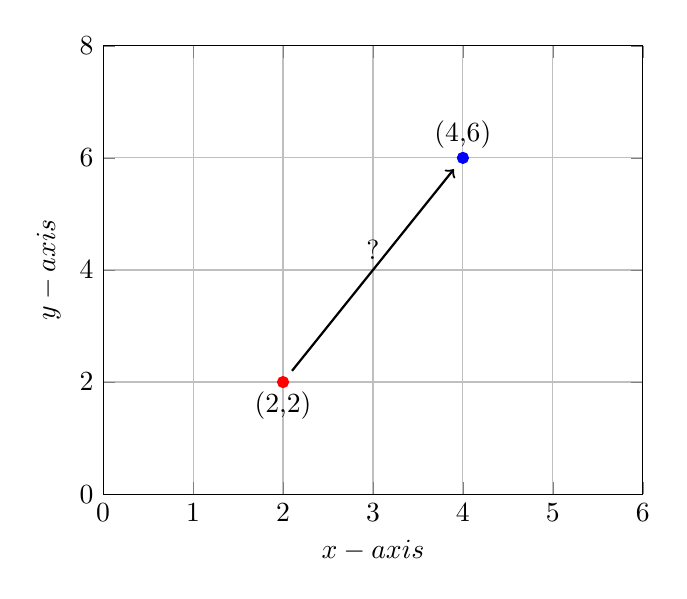
\begin{tikzpicture}
        \begin{axis}[
                      xlabel=$x-axis$,
                      ylabel=$y-axis$,
                      xmin=0, xmax=6,
                      ymin=0, ymax=8,
                      grid=both
                    ]
            \addplot[color=red, only marks]
                coordinates{
                    (2,2)
                };

            \node[below] at (axis cs: 2,2) {(2,2)};

            \addplot[color=blue, only marks]
                coordinates{
                    (4,6)
                };

            \node[above] at (axis cs: 4,6) {(4,6)};

            \draw[thick,->] (axis cs: 2.1,2.2) -- node[above]{?} (axis cs: 3.9,5.8);
        \end{axis}
    \end{tikzpicture}

    Notice that we are not interested in calculate the distance between this
    points, what we want to find is a number that decribes how much the thing's
    position has change when he moves from the beginning to the second possition.

    This can be done by calculating for each unit of distance that the object
    has move, how much the object assend. This calculus can be  described as
    follows

    \begin{equation}
        change = \frac{ascend}{advance}
    \end{equation}

    \vspace{1cm}

    For the example the formula would be $change = \frac{2}{1} = 2$, this
    means that every time that the thing moves 1 unit, also assend two units.
    Now the illustration \\

    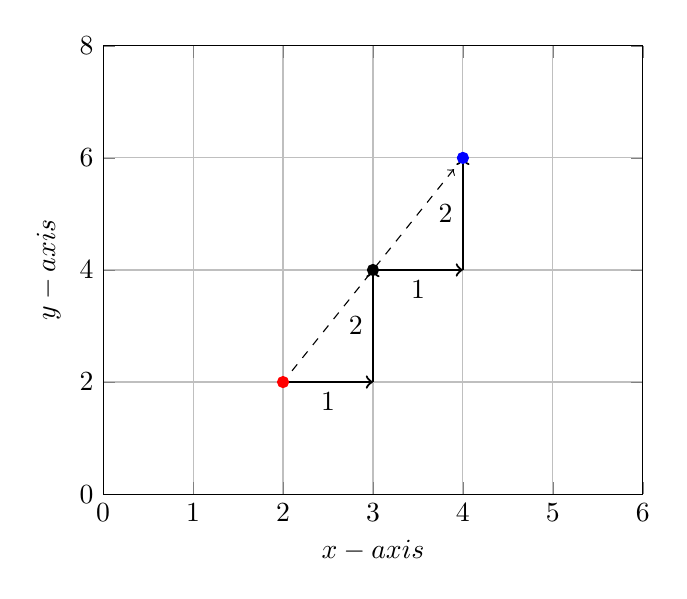
\begin{tikzpicture}
        \begin{axis}[
                      xlabel=$x-axis$,
                      ylabel=$y-axis$,
                      xmin=0, xmax=6,
                      ymin=0, ymax=8,
                      grid=both
                    ]
            \addplot[color=red, only marks]
                coordinates{
                    (2,2)
                };

            \addplot[color=black, only marks]
                coordinates{
                    (3,4)
                };

            \addplot[color=blue, only marks]
                coordinates{
                    (4,6)
                };

            \draw[dashed,->] (axis cs: 2.1,2.2) -- (axis cs: 3.9,5.8);

            \draw[thick,->] (axis cs: 2,2) -- node[below]{1} (axis cs: 3,2);
            \draw[thick,->] (axis cs: 3,2) -- node[left]{2} (axis cs: 3,4);

            \draw[thick,->] (axis cs: 3,4) -- node[below]{1} (axis cs: 4,4);
            \draw[thick,->] (axis cs: 4,4) -- node[left]{2} (axis cs: 4,6);
        \end{axis}
    \end{tikzpicture}

    Now that we know the "rate of change" of the movement we can calculate which
    would be the position of the object at any moment of the movement, this
    means that we can know the position when the object has move 1 unit, 2
    units, or any amount of units that we want.

    \begin{figure}[h!]
        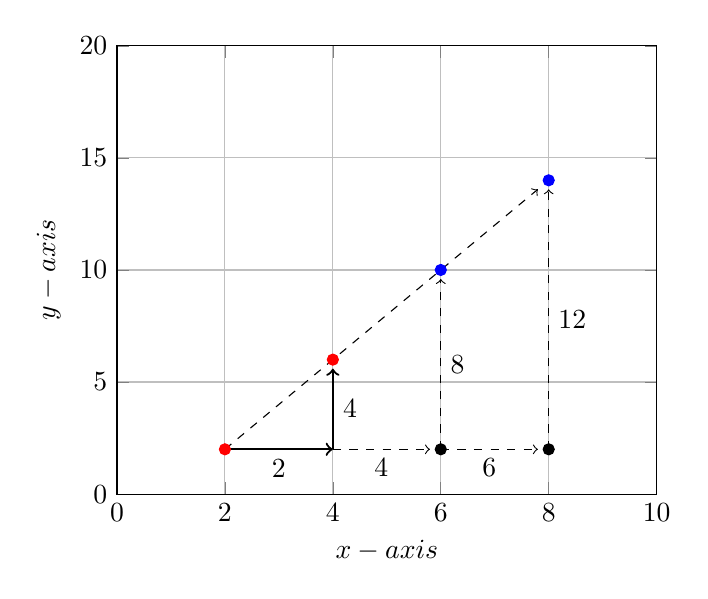
\begin{tikzpicture}
            \begin{axis}[
                          xlabel=$x-axis$,
                          ylabel=$y-axis$,
                          xmin=0, xmax=10,
                          ymin=0, ymax=20,
                          grid=both
                        ]
                \addplot[color=red, only marks]
                    coordinates{
                        (2,2)
                        (4,6)
                    };

                \addplot[color=blue, only marks]
                    coordinates{
                        (6,10)
                        (8,14)
                    };

                \addplot[color=black, only marks]
                    coordinates{
                        (6,2)
                        (8,2)
                    };

                \draw[thick,->] (axis cs: 2,2) -- node[below]{2} (axis cs: 4,2);
                \draw[thick,->] (axis cs: 4,2) -- node[right]{4} (axis cs: 4,5.6);

                \draw[dashed,->] (axis cs: 4,2) -- node[below]{4} (axis cs: 5.8,2);
                \draw[dashed,->] (axis cs: 6,2) -- node[right]{8} (axis cs: 6,9.6);

                \draw[dashed,->] (axis cs: 6,2) -- node[below]{6} (axis cs: 7.8,2);
                \draw[dashed,->] (axis cs: 8,2) -- node[right]{12} (axis cs: 8,13.6);

                \draw[dashed,->] (axis cs: 2,2) -- (axis cs: 7.8,13.6);
            \end{axis}
        \end{tikzpicture}
    \end{figure}

    This means that now we can predict how is going to be the movement of the
    object. All we have to do is take the units of movement that we want in the
    horizontal axis and then multiply that number for the change that we found
    before and thats all.\\

    Now we are going to formalize this concept a little bit. First we are going
    to change the name of the variable "change" to just a letter for simplicity,
    lets say "m". \\

    $change = m$ \\

    Now we are going to define the horizontal distance between the points
    as the difference between the two $x$ components and the vertical distance as
    the difference between the two $y$ components. In mathematics the difference
    between a same variable is denoted as $\Delta$variable, this means that the
    difference between the $x$ component will be $\Delta x$ and the difference
    between the $y$ components will be $\Delta y$\\

    \begin{tikzpicture}
        \begin{axis}[
                      xlabel=$x-axis$,
                      ylabel=$y-axis$,
                      xmin=0, xmax=7,
                      ymin=0, ymax=8,
                      xtick=\empty,
                      ytick=\empty,
                    ]
            \addplot[color=red, only marks]
                coordinates{
                    (2,2)
                };
            \node[above] at (axis cs: 2,2) {($x_1$,$y_1$)};

            \addplot[color=blue, only marks]
                coordinates{
                    (4,6)
                };
            \node[left] at (axis cs: 4,6) {($x_2$,$y_2$)};

            \draw[thick] (axis cs: 2,2) -- node[below]{$x_2 - x_1 = \Delta x$}(axis cs: 4,2);
            \draw[thick] (axis cs: 4,2) -- node[right]{$y_2 - y_1 = \Delta y$} (axis cs: 4,6);
        \end{axis}
    \end{tikzpicture}

    Then we can define the change as follows

    \begin{equation}
        m = \frac{\Delta y}{\Delta x}
    \end{equation}

    The last formula is the formal definition of the slope in mathematics, this
    is the change of state in a point of a linear function, just like we have
    explained earlier.

    This works very good for any linear function, but what happens when we
    want to analise a non linear function like a curve?. Lets analize an
    example, we are goint to take a fuction with a curve graphic, we are going to
    take a point and we want to calculate the change in that specific point,
    this can be achived by finding the value of the slope in that point, in other
    words finding the rate of change in that specific point.

    The problem is that we only know how to calculate the slope with two points,
    so we are goint to take a second point with reference to the original point,
    this difference is goint to be a number called "$h$" \\

    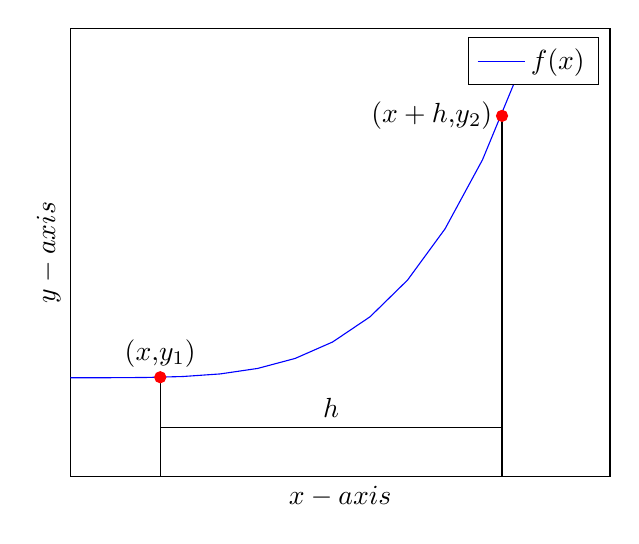
\begin{tikzpicture}
        \begin{axis}[
                      xlabel=$x-axis$,
                      ylabel=$y-axis$,
                      xmin=0, xmax=6,
                      ymin=-200,
                      xtick=\empty,
                      ytick=\empty
                    ]

            \addplot[color=blue]{x^4};
            \addlegendentry{$f(x)$}

            \addplot[color=red, only marks]
                coordinates{
                    (1,1)
                };
            \node[above] at (axis cs: 1,1) {($x$,$y_1$)};


            \addplot[color=red, only marks]
                coordinates{
                    (4.8,530)
                };
            \node[left] at (axis cs: 4.8,530) {($x+h$,$y_2$)};

            \draw (axis cs: 1,-200) -- (axis cs: 1,1);
            \draw (axis cs: 4.8,-200) -- (axis cs: 4.8,530);
            \draw (axis cs: 1,-100) -- node[above]{$h$} (axis cs: 4.8,-100);
        \end{axis}
    \end{tikzpicture}

    Notice that those points are part of a function, this means that the high
    of any point in the graphic can be calculated as the function evaluated in
    the point of the $x$ axis that we want to evaluate. Now an example \\

    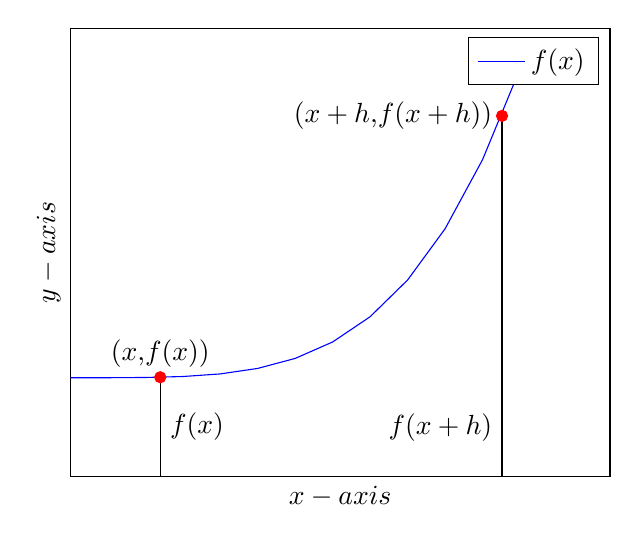
\begin{tikzpicture}
        \begin{axis}[
                      xlabel=$x-axis$,
                      ylabel=$y-axis$,
                      xmin=0, xmax=6,
                      ymin=-200,
                      xtick=\empty,
                      ytick=\empty
                    ]

            \addplot[color=blue]{x^4};
            \addlegendentry{$f(x)$}

            \addplot[color=red, only marks]
                coordinates{
                    (1,1)
                };
            \node[above] at (axis cs: 1,1) {($x$,$f(x)$)};


            \addplot[color=red, only marks]
                coordinates{
                    (4.8,530)
                };
            \node[left] at (axis cs: 4.8,530) {($x+h$,$f(x +h)$)};

            \draw (axis cs: 1,-200) -- node[right]{$f(x)$} (axis cs: 1,1);
            \draw (axis cs: 4.8,-200) -- (axis cs: 4.8,530);

            \node[left] at (axis cs: 4.8,-100) {$f(x+h)$};
        \end{axis}
    \end{tikzpicture}

    Now with this new concepts we can define the slope of this two points as

    \begin{equation}
        m = \frac{f(x+h) - f(x)}{(x+h) - x}
    \end{equation}

    We can simplify the last equation

    \begin{equation}
        m = \frac{f(x+h) - f(x)}{h}
    \end{equation}

    Now with this new formula we can calculate the slope of the two points and
    find the line that cross the points.

    Regrettably this slope does not describe the change of the point very well
    because the line does not touch the function in just one point (this is
    what a tangent line is), insted touch the function two times (this is call a
    secant line), this means that the change of the point that we are
    calculating is taking into account two points of the function, not only the
    original point, so this is not what we want. Now the ilustration \\

    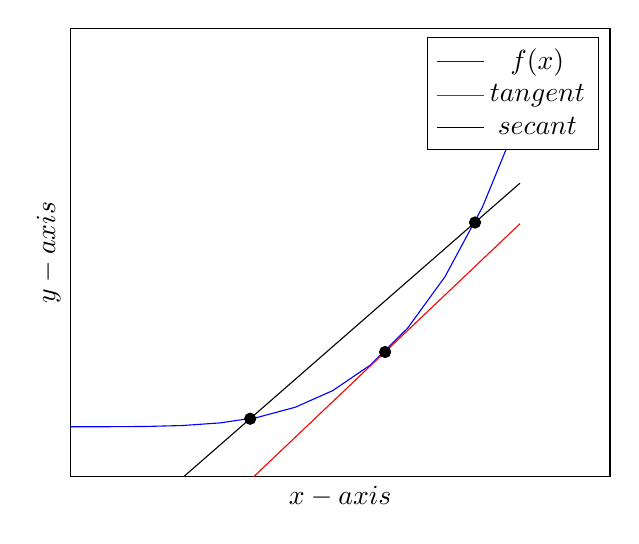
\begin{tikzpicture}
        \begin{axis}[
                      xlabel=$x-axis$,
                      ylabel=$y-axis$,
                      xmin=0, xmax=6,
                      ymin=-100, ymax=800,
                      xtick=\empty,
                      ytick=\empty,
                    ]

            \addplot[color=blue]{x^4};
            \addlegendentry{$f(x)$}

            \addplot[color=red]{171.5*x-450};
            \addlegendentry{$tangent$}

            \addplot[color=black]{157.6*x-299};
            \addlegendentry{$secant$}

            \addplot[color=black, only marks]
                coordinates{
                    (3.5,150)
                    (2,16)
                    (4.5,410)
                };

        \end{axis}
    \end{tikzpicture}

    Until this moment we have the following graphic \\

    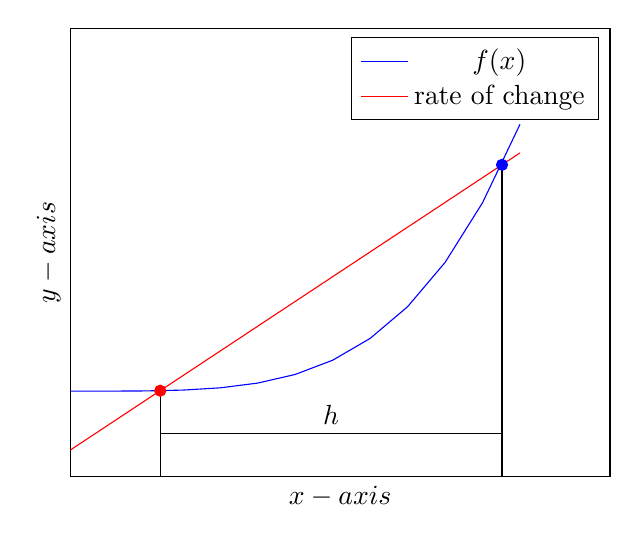
\begin{tikzpicture}
        \begin{axis}[
                      xlabel=$x-axis$,
                      ylabel=$y-axis$,
                      xmin=0, xmax=6,
                      ymin=-200, ymax=850,
                      xtick=\empty,
                      ytick=\empty
                    ]

            \addplot[color=blue]{x^4};
            \addlegendentry{$f(x)$}

            \addplot[color=red]{139.2*x-138};
            \addlegendentry{rate of change}

            \addplot[color=red, only marks]
                coordinates{
                    (1,1)
                };

            \addplot[color=blue, only marks]
                coordinates{
                    (4.8,530)
                };

            \draw (axis cs: 1,-200) -- (axis cs: 1,1);
            \draw (axis cs: 4.8,-200) -- (axis cs: 4.8,530);
            \draw (axis cs: 1,-100) -- node[above]{$h$} (axis cs: 4.8,-100);
        \end{axis}
    \end{tikzpicture}

    What happens if we start to make $h$ smaller?, the points will be closser
    every time, so the linear function is going to start be much more closer
    to predict the correct rate of change of the point that we are analyzing,
    in other words the secant line that we have will tend to be a tangent, just
    as we want. Here the ilustration

    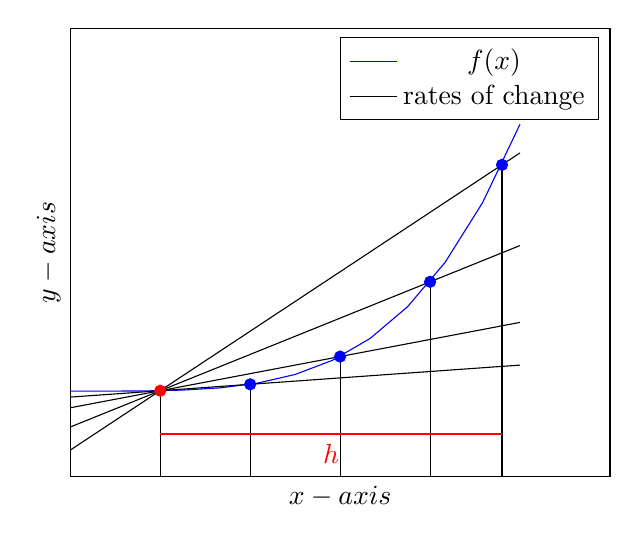
\begin{tikzpicture}
        \begin{axis}[
                      xlabel=$x-axis$,
                      ylabel=$y-axis$,
                      xmin=0, xmax=6,
                      ymin=-200, ymax=850,
                      xtick=\empty,
                      ytick=\empty
                    ]

            \addplot[color=blue]{x^4};
            \addlegendentry{$f(x)$}

            \addplot[color=black]{139.2*x-138};
            \addlegendentry{rates of change}

            \addplot[color=black]{85*x-84};
            \addplot[color=black]{40*x-39};
            \addplot[color=black]{15*x-14};

            \addplot[color=red, only marks]
                coordinates{
                    (1,1)
                };

            \addplot[color=blue, only marks]
                coordinates{
                    (4.8,530)
                    (4,256)
                    (3,81)
                    (2,16)
                };

            \draw (axis cs: 1,-200) -- (axis cs: 1,1);
            \draw (axis cs: 4.8,-200) -- (axis cs: 4.8,530);
            \draw (axis cs: 4,-200) -- (axis cs: 4,256);
            \draw (axis cs: 3,-200) -- (axis cs: 3,81);
            \draw (axis cs: 2,-200) -- (axis cs: 2,16);

            \draw[thick, color=red] (axis cs: 1,-100) -- node[below]{$h$} (axis cs: 4.8,-100);
        \end{axis}
    \end{tikzpicture}

    Is for this reason that the derivative is define as follows

    \begin{equation}
        \lim_{h \to 0} \frac{f(x+h) - f(x)}{h}
    \end{equation}

    Finally this is the formal definition of a derivative, if we apply this
    concept to the previus graphics we can get directly the tanget line that
    pass through a specific point of a function and the slope or rate of change
    of that point. \\

    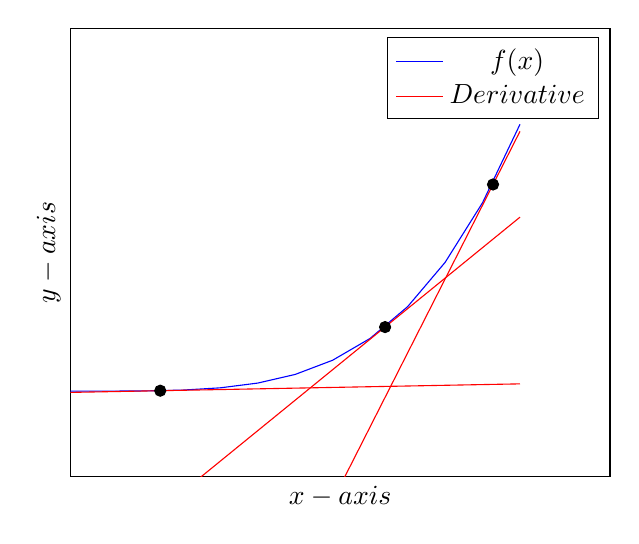
\begin{tikzpicture}
        \begin{axis}[
                      xlabel=$x-axis$,
                      ylabel=$y-axis$,
                      xmin=0, xmax=6,
                      ymin=-200, ymax=850,
                      xtick=\empty,
                      ytick=\empty
                    ]

            \addplot[color=blue]{x^4};
            \addlegendentry{$f(x)$}

            \addplot[color=red]{4*x-3};
            \addlegendentry{$Derivative$}

            \addplot[color=red]{171.5*x-450};
            \addplot[color=red]{415.3*x-1468};

            \addplot[color=black, only marks]
                coordinates{
                    (1,1)
                    (3.5,150)
                    (4.7,484)
                };
        \end{axis}
    \end{tikzpicture}

    As we can see in the last graphic the slope of the first point is almost
    horizontal, this means that the rate of change is samall, in the second
    is bigger and in the third point is the most vertical, so is the point with
    the highest change in the graphic, just like it would be, so we can
    conclude that with the derivative we can know the rate of change the
    functions at any point (almost, see defferentiable functions for more
    information).

\end{document}
